\documentclass[12pt,a4paper]{article}

% Packages essentiels
\usepackage[utf8]{inputenc}
\usepackage[T1]{fontenc}
\usepackage[french]{babel}
\usepackage{amsmath}
\usepackage{amsfonts}
\usepackage{amssymb}
\usepackage{graphicx}
\usepackage[hidelinks]{hyperref}
\usepackage{geometry}
\usepackage{float}

% Configuration de la géométrie de la page
\geometry{
    a4paper,
    margin=2.5cm
}

% Informations du document
\title{Compte-Rendu : Transformée de Radon Fenêtrée et\\Décomposition Tensorielle de Rang 1 pour le\\Beamforming Adaptatif en Échographie Ultrarapide}
\author{CADET Florent}
\date{\today}

\begin{document}

\pagenumbering{gobble}
\maketitle

\begin{abstract}
Ce compte-rendu analyse une nouvelle approche de beamforming adaptatif pour l'imagerie ultrasonore ultrarapide, basée sur la combinaison de la transformée de Radon fenêtrée et de la décomposition tensorielle de rang 1. Cette méthode permet une correction efficace des aberrations de phase tout en maintenant une excellente résolution d'image.
\end{abstract}

\clearpage
\pagenumbering{arabic}
\tableofcontents

\clearpage
\section{Analyse de la Méthode Proposée}

La méthode présentée dans l'article introduit une approche novatrice pour le beamforming adaptatif en échographie ultrarapide. L'innovation principale réside dans la combinaison de deux techniques : la transformée de Radon fenêtrée et la décomposition tensorielle de rang 1. Cette approche permet de corriger simultanément les aberrations en émission et en réception, tout en préservant la parallélisation des calculs, comme illustré dans la Figure 1 des annexes. Le pipeline de traitement comprend une segmentation des données en patches, suivie d'une analyse par transformée de Radon fenêtrée et d'une décomposition tensorielle, avant la reconstruction finale de l'image.

\subsection{Avantages de l'Approche}
La méthode développée présente plusieurs avantages significatifs par rapport aux techniques existantes. La correction simultanée des aberrations en émission et réception constitue une amélioration majeure, permettant une meilleure reconstruction des images échographiques. La parallélisation efficace des calculs, rendue possible par l'architecture proposée, optimise les temps de traitement. Les résultats présentés en Figure 2 démontrent une amélioration notable de la résolution des diffuseurs et une augmentation significative du contraste des images par rapport aux méthodes conventionnelles.

\subsection{Résultats Principaux}
L'analyse quantitative des performances, détaillée dans la Figure 3, révèle l'influence cruciale du paramètre de régularisation μ sur la qualité des images reconstruites. Pour les inclusions anéchoïques, le contraste atteint -32 dB, tandis que les inclusions hypoéchoïques sont mieux définies avec un contraste de -7 dB. La résolution spatiale montre également une amélioration significative, avec une réduction de la FWHM des diffuseurs entre 200 et 600 μm, comme le montre la Figure 4 qui présente une analyse détaillée des structures reconstruites.

L'étude de l'impact du nombre d'insonifications, présentée en Figure 5, démontre la robustesse de la méthode même avec un nombre réduit d'émissions. Cette caractéristique est particulièrement importante pour les applications nécessitant une cadence d'imagerie élevée. Les tests sur fantôme in-vitro, illustrés en Figure 6, confirment la capacité de la méthode à gérer différents niveaux d'aberration, avec une performance maintenue jusqu'à des délais d'aberration significatifs.

La validation in-vivo, présentée en Figure 7, démontre l'applicabilité clinique de la méthode. Les images de la paroi abdominale montrent une amélioration notable de la définition des structures anatomiques, avec une meilleure délimitation des interfaces tissulaires et une réduction des artefacts d'aberration. Cette amélioration est particulièrement visible dans les zones profondes de l'image, où les effets des aberrations sont traditionnellement plus prononcés.

\section{Conclusion}
Cette nouvelle approche représente une avancée significative dans le domaine du beamforming adaptatif. Les résultats quantitatifs démontrent sa supériorité par rapport aux méthodes existantes, particulièrement en termes de contraste et de résolution. La méthode offre également un contrôle précis du compromis entre qualité d'image et robustesse via son paramètre de régularisation, ouvrant la voie à des applications cliniques prometteuses. L'ensemble des validations, tant sur données simulées qu'in-vivo, confirme le potentiel de cette approche pour améliorer la qualité diagnostique de l'imagerie échographique ultrarapide.

\clearpage
\appendix
\section{Annexes : Illustrations et Résultats}

\subsection{Méthodologie et Pipeline de Traitement}
\begin{figure}[H]
    \centering
    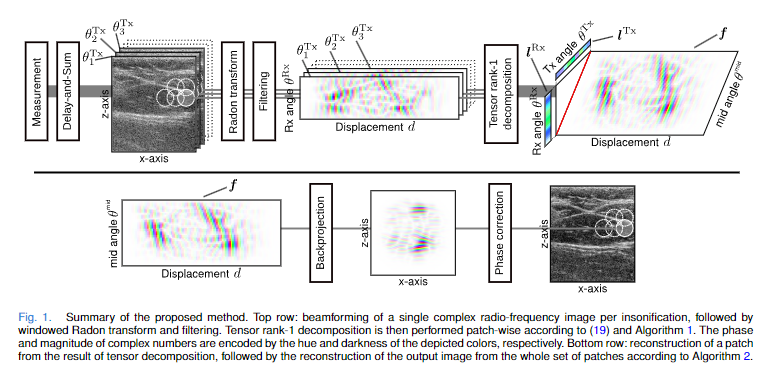
\includegraphics[width=0.95\textwidth]{paper/fig_1.png}
    \caption{Vue d'ensemble de la méthode proposée : (haut) étapes de beamforming et transformée de Radon fenêtrée, (bas) reconstruction d'image à partir des patches traités.}
\end{figure}

\subsection{Évaluation sur Fantôme Numérique}
\begin{figure}[H]
    \centering
    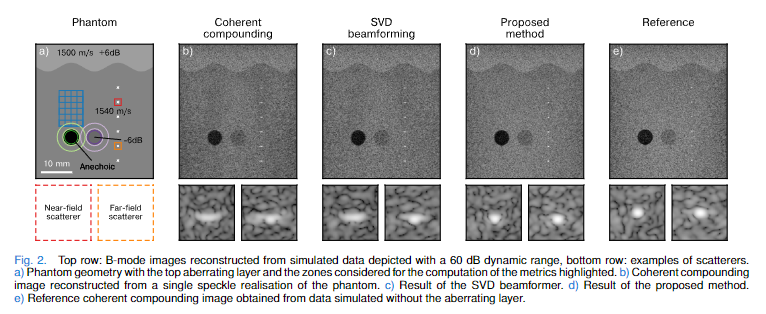
\includegraphics[width=0.95\textwidth]{paper/fig_2.png}
    \caption{Résultats sur fantôme numérique : (a) Géométrie du fantôme avec zones d'analyse, (b) Compounding cohérent, (c) Beamforming SVD, (d) Méthode proposée, (e) Image de référence sans aberration.}
\end{figure}

\subsection{Analyse des Performances}
\begin{figure}[H]
    \centering
    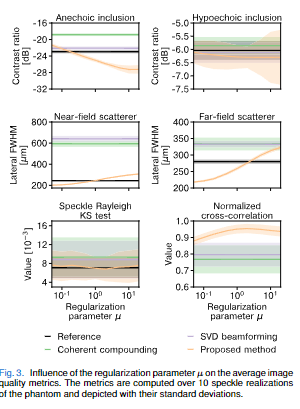
\includegraphics[width=0.95\textwidth]{paper/fig_3.png}
    \caption{Influence du paramètre de régularisation μ sur les métriques de qualité d'image : contraste des inclusions, résolution des diffuseurs, statistiques du speckle et corrélation avec l'image de référence.}
\end{figure}

\subsection{Analyse Détaillée des Structures}
\begin{figure}[H]
    \centering
    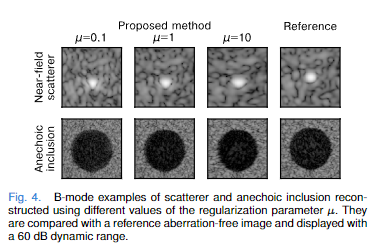
\includegraphics[width=0.95\textwidth]{paper/fig_4.png}
    \caption{Exemples de reconstruction de diffuseurs et d'inclusions avec différentes valeurs du paramètre de régularisation μ, comparés à l'image de référence.}
\end{figure}

\subsection{Impact du Nombre d'Insonifications}
\begin{figure}[H]
    \centering
    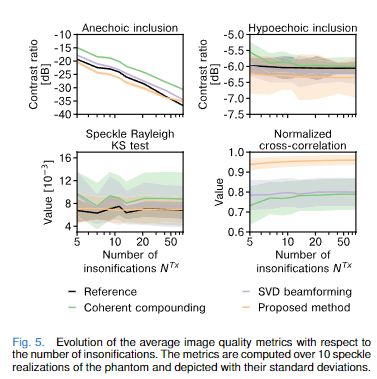
\includegraphics[width=0.95\textwidth]{paper/fig_5.png}
    \caption{Évolution des métriques de qualité d'image en fonction du nombre d'ondes planes émises, montrant la robustesse de la méthode même avec peu d'insonifications.}
\end{figure}

\subsection{Validation In-Vitro}
\begin{figure}[H]
    \centering
    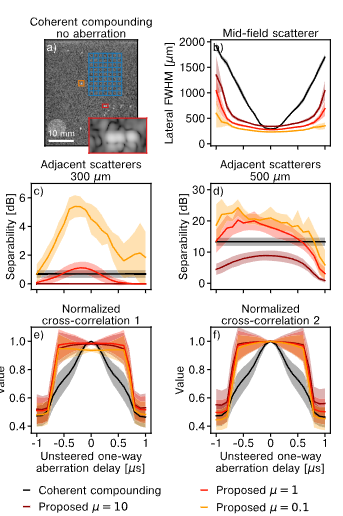
\includegraphics[width=0.95\textwidth]{paper/fig_6.png}
    \caption{Résultats sur fantôme in-vitro : (a) Image de référence avec zones d'analyse, (b-f) Métriques de performance en fonction du délai d'aberration.}
\end{figure}

\subsection{Validation In-Vivo}
\begin{figure}[H]
    \centering
    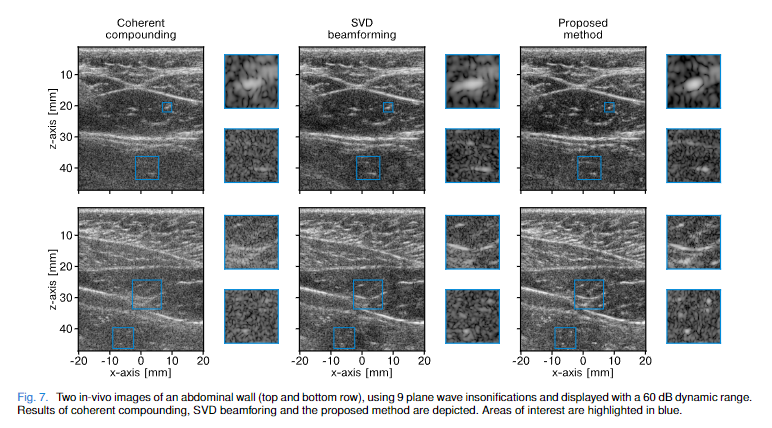
\includegraphics[width=0.95\textwidth]{paper/fig_7.png}
    \caption{Images in-vivo de la paroi abdominale obtenues avec différentes méthodes de reconstruction, démontrant l'amélioration de la qualité d'image dans un contexte clinique.}
\end{figure}

\end{document} 